Un sistema dinamico può essere descritto, a livello intuitivo, come un sistema fisico il cui stato evolve nel tempo.
\section{Definire un Sistema dinamico}%
\label{sub:Sistema dinamico Deterministico e Stocastico.}
Prendiamo un insieme $X$\sidenote{\scriptsize Che definiremo avanti come \textit{Spazio degli stati}, \textit{Spazio degli eventi} o \textit{Spazio delle fasi}.} 
, lo stato $x$ di un sistema al tempo iniziale è definito da $x_0 = x(t=0)$
\leavevmode\marginpar{
    \captionsetup{type=figure}
        \incfig{1_1}
    \caption{\scriptsize Evoluzione temporale \textit{deterministica} di $x$ all'interno di $X$.}
    \label{fig:1_1}
}.
\begin{defn}[Sistema Dinamico Deterministico]
    Un sistema dinamico si dice deterministico quando la sua evoluzione temporale segue regole deterministiche.
\end{defn}
\noindent
In Figura \ref{fig:1_1} abbiamo un esempio di sistema dinamico con evoluzione deterministica.\\
Prendiamo un altro sistema preparato ad un istante iniziale in $x_0$. Se al tempo $t$ il sistema è caratterizzato da una certa probabilità di trovarsi in $x$ \sidenote{\scriptsize $P$ diversa dalla distribuzione $\delta(x)$, altrimenti il processo è deterministico!}
allora il Sistema Dinamico si dice stocastico (o processo stocastico).\\
Un processo stocastico $\vect{x} \in \mathbb{R}^n$ è caratterizzato da due parametri: $\vect{x} (t, \omega)$. Il primo indica il tempo, il secondo è legato alla parte stocastica del processo. \\
Il parametro $\omega$ appartiene allo spazio degli eventi $\Omega$:
\[
    \omega  \in \Omega
.\] 
Significa che $ \forall \ \omega^* \in \Omega$ corrisponde un punto $\vect{x} (t, \omega^*)$ che è definito come la \textit{realizzazione di }$\omega^*$.
\marginpar{
    \captionsetup{type=figure}
        \incfig{1_2}
    \caption{\scriptsize Evoluzione 1D di processo stocastico date le condizioni iniziali $x_0$.}
    \label{fig:1_2}
}
\begin{defn}[Processo stocastico]
    Collezione di funzioni $\forall \ t$ al variare di $\omega$ nello spazio degli eventi.
\end{defn}
\noindent
\subsection{Rappresentazione di un Sistema Dinamico}%
\label{sub:Rappresentazione di un Sistema Dinamico}
\paragraph{Sistema dinamico a tempo continuo.}%
\label{par:Sistema dinamico a tempo continuo.}
Un SD a tempo continuo è rappresentato in generale da un sistema di equazioni differenziali:
\[
    \frac{\text{d} \vect{x}}{\text{d} t} = F(\vect{x}, t, \vect{u});
    \qquad 
    \vect{x}\in U \subset \mathbb{R}^n, \ \vect{u}  \in \mathbb{R}^p
.\] 
La funzione $F$ è definita nel seguente dominio:
\[
    F: \ U \times I \times \Gamma  \to V \subset \mathbb{R}^n
.\] 
\begin{itemize}
    \item $U$ è il dominio della funzione $\vect{x}$.
    \item $I$ è l'intervallo di definizione della soluzione (non ché l'intervallo temporale studiato).
    \item $\Gamma$ è il sottospazio dell'insieme dei parametri $\mathbb{R}^p$.
    \item $V$ L'insieme in cui viene mappato il dominio iniziale dalla $F$.
\end{itemize}
\begin{defn}[Notazione semplificata]
    Nel seguito si sceglie di alleggerire la notazione dei sottospazi. Abuseremo del termine $\mathbb{R}$ per definire tutti gli spazi
    \[
        U, I, \Gamma, V
    .\] 
    Con l'opportuna dimensionalità.
\end{defn}
\noindent
Sarà \textbf{importante} saper ricostruire i giusti insiemi di definizione di tutti i termini per i casi di studio analizzati.
\paragraph{Sistemi di equazioni differenziali}%
\label{par:Sistemi di equazioni differenziali}
Una equazione differenziale è definita dalla seguente:
\begin{equation}
    E\left(\frac{\text{d} ^n x}{\text{d} t^n} , \ldots, \frac{\text{d} x}{\text{d} t}, x, t\right) = 0 
    \qquad
    x \in \mathbb{R}, \ t \in \mathbb{R}
    \label{eq:1_eq_diff}
\end{equation}
In cui si fa uso della notazione semplificata. Il grado di una equazione differenziale è l'ordine massimo delle sue derivate ($n$ in questo caso).\\
Se è possibile riscrivere la \ref{eq:1_eq_diff} isolando il termine di ordine $n$:
\[
    \frac{\text{d}^n x}{\text{d} t^n} = G\left(\frac{\text{d} ^{n-1}x}{\text{d} t^{n-1}} , \ldots, x, t\right)
.\] 
Allora l'equazione differenziale iniziale è scomponibile in $n$  equazioni differenziali del primo ordine con il seguente cambio di variabili:
\[
    y_1(t) = x(t); \quad \ldots \quad y_n(t) = \frac{\text{d} ^{n-1}x}{\text{d} t^{n-1}} 
.\] 
Quindi è possibile definire un nuovo vettore di $\mathbb{R}^n$:
\[
    \vect{y}  = (y_1, y_2, \ldots, y_n) \in \mathbb{R}^n
.\] 
In conclusione il sistema da risolvere è:
\[\begin{aligned}
    & \frac{\text{d} y_1}{\text{d} t} = y_2\\
    & \frac{\text{d} y_2}{\text{d} t} = y_3\\
    & \vdots\\
    & \frac{\text{d} y_n}{\text{d} t} = G(y_n, y_{n-1}, \ldots, y_1, t)
.\end{aligned}\]
\begin{exmp}[SD a tempo continuo: Oscillatore armonico]
    Prendiamo un sistema descritto dalla seguente Hamiltoniana:
    \[
        H = \frac{1}{2}ky_1^2 + \frac{1}{2}m y_2^2
    .\] 
    In questo caso lo stato del sistema è descritto dalla variabile $\vect{x}$:
    \[
	\vect{x}(t) = (y_1, y_2)
    .\] 
    Il sistema è conservativo: fissate le condizioni iniziali la quantità $H$ è conservata, questo di fatto significa che l'energia è conservata.
    \[
        E = \frac{1}{2}ky_1^2 + \frac{1}{2}m y_2^2 = \text{cost}
    .\] 
    Di conseguenza lo spazio delle fasi (o spazio degli stati) è definito in \textit{un sottoinsieme di }$\mathbb{R}^2$: un'ellisse.
    \marginpar{
        \captionsetup{type=figure}
            \incfig{1_3}
	    \caption{\scriptsize Spazio delle fasi con una soluzione per il sistema Hamiloniano (a tempo continuo).}
        \label{fig:1_3}
    }
    \[
        \frac{y_1^2}{2E /k} + \frac{y_2^2}{2E /m} = 1
    .\] 
    I semiassi dell'ellisse sono:
    \[
        a^2 = \frac{2E}{k} \qquad b^2 = \frac{2E}{m}
    .\] 
    Notiamo che l'orbita nello spazio delle fasi è chiusa: il sistema è periodico.
\end{exmp}
\noindent
\begin{defn}[Spazio delle fasi]
    Sottoinsieme di $\mathbb{R}^n$ con le soluzioni (gli stati).
\end{defn}
\noindent
\paragraph{Sistema dinamico a tempo discreto}%
\label{par:Sistema dinamico a tempo discreto}
Una prima rappresentazione di SD a tempo discreto\sidenote{\scriptsize Valida per i sistemi dinamici "fisici" che studieremo, più tardi daremo anche una definizione più generale ed astratta.}
è la seguente:
\[
    \vect{x}_n = G(\vect{x}_{n-1}, \vect{u}); \qquad \vect{x}_n \in U \subset \mathbb{R}^n, \ \vect{u}  \in \mathbb{R}^p
.\] 
\[
    G: \ U\times \mathbb{R}^p \to V \subset \mathbb{R}^n
.\] 
Possiamo immaginare che tra lo step $n$ e lo step $n-1$ vi sia un intervallo temporale $\Delta t$. Fisicamente può essere la distanza tra due osservazioni sperimentali oppure l'andamento giornaliero di una popolazione. \\
Ovviamente l'intervallo $\Delta t$ dipende dal contesto e dal tipo di sistema sotto esame.
\begin{exmp}[Osservazione delle macchie solari.]
    \marginpar{
        \captionsetup{type=figure}
	\fbox{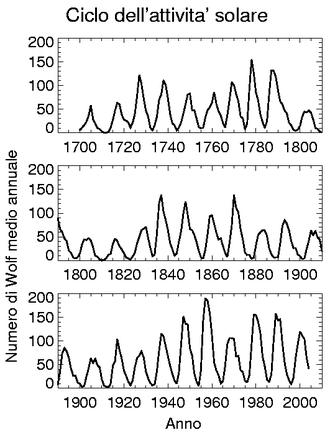
\includegraphics[width=\marginparwidth]{figures/1_4_macchie.png}}
	\caption{\scriptsize Andamento delle macchie solari (wikipedia).}
        \label{fig:1_4_macchie-png}
    }
    Un SD a tempi discreti può essere realizzato con l'osservazione delle macchie solari ogni 6 mesi. \\
    Nella pratica si ottengono degli andamenti come in Figura \ref{fig:1_4_macchie-png}.
\end{exmp}
\noindent
\begin{exmp}[Andamento degli individui di una popolazione, modello lineare.]
    \label{ex:pop_lin}
   Prendiamo una popolazione di individui descritta dallo stato $N_i$: il numero di individui al tempo $t=i \ \in \mathbb{N}$. \\
   La dinamica dello stato è descritta dal legame tra $N_i$ e $N_{i-1}$. Nota questa legge è possibile predire i futuri andamenti della popolazione.\\
   Il modello più semplice da studiare è il \textbf{modello lineare}:
   \[
       N_n = r N_{n-1} \qquad r \in \mathbb{R}^+
   .\] 
   Ipotizzando che il numero di individui all'istante iniziale (arbitrario) sia $N_0$ è possibile ricostruire una legge temporale che lega l'istante iniziale all'istante $n$:
   \[
       N_1 = rN_0; \qquad N_2 = rN_1=r^2N_0 \qquad \implies \qquad N_n = r^{n}N_0
   .\] 
   Quindi lo stato $n$-esimo è definito tramite una \textit{rete deterministica} legata allo stato iniziale.
   \marginpar{
       \captionsetup{type=figure}
           \incfig{1_5}
       \caption{\scriptsize Andamento della soluzione $N$ al variare del parametro $r$.}
       \label{fig:1_5}
   }
   Dalla Figura \ref{fig:1_5} si può osservare come l'andamento delle soluzioni dipende esclusivamente dal parametro $r$: sono possibili soltanto 3 casi.\\
   Il modello lineare è il più semplice che si possa costruire per studiare le popolazioni e, per quasi tutti i casi, non basta a spiegare i fenomeni fisici che ci circondano: è necessario elaborare un modello più complesso\ldots
\end{exmp}
\noindent
\paragraph{Principio di sovrapposizione}%
\label{par:Principio di sovrapposizione}
Riprendiamo l'Esempio \ref{ex:pop_lin}, abbiamo concluso che l'andamento dello stato del sistema (la popolazione) seguiva la legge:
\[
    N_n = r^nN_0
.\] 
Ipotizziamo che l'analisi prenda in considerazione l'andamento di due distinte popolazioni che seguono tale legge:
\[
    N_n = r^nN_0; \qquad M_n = r^nM_0
.\] 
Se lo studio prevede che queste due popolazioni si uniscano\sidenote{\scriptsize ad esempio per qualche ragione fisica, come la convivenza sullo stesso territorio} allora si ottiene la nuova popolazione $\overline{N}$:
\[
    \overline{N}_n = N_n + M_n = r^n(N_n + M_n) = r^n \overline{N}
.\] 
\begin{thm}[Principio di sovrapposizione.]
    Dati due sistemi che evolvono linearmente con la stessa legge: l'evoluzione della somma dei due ha lo stesso andamento della evoluzione dei singoli. 
\end{thm}
\noindent
Cosa avviene se i due sistemi non evolvono linearmente?
\subsection{Introduzione al Modello Logistico}%
\label{sub:Introduzione al Modello Logistico}
Prendiamo il seguente modello di popolazione:
\[
    N_{n+1} = r(N_n)\cdot N_n
.\] 
A differenza dell'esempio \ref{ex:pop_lin} il rate della popolazione $r$ adesso non è costante: dipende dalla popolazione all'istante $n$.\\
Un caso particolare di questa classe di sistemi è stato al centro di molti studi, in particolare per la sua versatilità nel modellizzare sistemi in ogni branca scientifica:
\begin{defn}[Modello logistico]
    Il modello logistico descrive l'andamento di una popolazione $N_n$ con il seguente rate $r$:
    \marginpar{
        \captionsetup{type=figure}
            \incfig{1_6}
        \caption{\scriptsize Andamento del Rate in funzione della popolazione, notiamo l'antimonotonia di $r$ che garantisce il fenomeno di retroazione.}
        \label{fig:1_6}
    }
    \[
	r(N_n) = \mu\left(1-\frac{N_n}{k}\right) 
    .\] 
    Quindi lo stato del sistema si esprime con la legge:
    \[
        N_{n+1} = \mu\left(1-\frac{N_n}{k}\right)N_n
    .\] 
    Questo rappresenta un modello non lineare.
\end{defn}
\noindent
Nel modello logistico la dipendenza di $r$ dalla popolazione permette un meccanismo di retroazione che sfavorisce la crescita della popolazione stessa.
\begin{exmp}[Modello logistico a popolazioni stellari.]
    Il modello logistico può essere utilizzato come "toy model" per descrivere il fenomeno di formazione delle stelle del tipo "Supernovae Triggered": 
    stelle che nascono in seguito all'esplosione di supernovae. \\
    Il modello prevede che le stelle neonate si trasformino in supernovae (al termine della loro vita) diventando anche loro sorgenti di stelle.
    \marginpar{
        \captionsetup{type=figure}
            \incfig{1_7}
        \caption{\scriptsize Porzione di spazio considerata per il modello, la stella con il contorno rosso è una stella in procinto di esplodere. $M$ è la quantità di materia totale all'interno di tale spazio, composta da stelle formate e gas interstellare.}
        \label{fig:1_7}
    }\\
    Ipotizziamo che ad un istante $i$ la popolazione di stelle sia $S_i$ e la massa del gas interstellare sia $M$. Tutte le stelle del modello hanno la stessa massa $m$ e sono identiche. \\
    Vogliamo modellare la popolazione stellare ad un istante successivo: $i+1$.\\
    La quantità di gas insterstellare disponibile (per la formazione di altre stelle) al tempo $t$ è data dalla massa totale $M$ meno la massa delle stelle presenti in tale istante:
    \[
        m_{\text{gas}} = M-S_i\cdot m
    .\] 
    Quindi il numero di stelle al tempo $i+1$ può essere espresso tramite un modello logistico:
    \[
	S_{i+1} = cS_i (M-S_i\cdot m)
    .\] 
    Cambiando variabili si arriva ad un sistema avente una notazione "classica" nello studio dei modelli logistici:
    \[
	x_i = \frac{mS_i}{M} \qquad r = \frac{cM}{4} \qquad \implies  \qquad x_{i+1} = 4rx_i(1-x_i)
    .\] 
\end{exmp}
\noindent
\subsection{Definizione Formale di Sistema Dinamico}%
\label{sub:Definizione Formale di Sistema Dinamico}
\paragraph{Spazio metrico}%
\label{par:Spazio metrico}
Prima di generalizzare le definizioni si SD è necessario definire uno spazio metrico:
\begin{defn}[Spazio metrico]
    L'inseme $X$ è spazio metrico se $\exists \ d:$ 
    \[
        d: \ X\times X \to \mathbb{R}^+ \cup \left\{0\right\}
    .\] 
    Che soddisfa le seguenti proprietà:
    \[\begin{aligned}
	& d(x, y) \ge 0; && \qquad d(x, y) = d(y, x); \\
	& d(x, y) = 0 \iff x = y; && \qquad d(x, y) \le d(x, z) + d(z, y)
    .\end{aligned}\]
\end{defn}
\noindent
\begin{exmp}[Spazio metrico]
    Prendiamo l'insieme di funzioni:
    \[
	C(I) = \left\{f(x)| x \in I \subset \mathbb{R}; f \text{ continua}\right\}
    .\] 
    Possiamo definire una distanza $d$ come:
    \[
	d(f(x), g(x)) = \sup\limits_{x \in I}\left|f(x)- g(x)\right|
    .\] 
\end{exmp}
\noindent
\paragraph{Definizione di SD a tempo discreto}%
\label{par:Definizione di SD a tempo discreto}
\begin{defn}[SD a tempo discreto]
    Un sistema dinamico a tempo discreto è rappresentato da una mappa $G: X\to X$ tale che
    \begin{itemize}
        \item $G^{n+m} = G^n \circ G^m \ \forall n, m \in \mathbb{N}_0 \cup \left\{0\right\}$.
	\item Se $G$ è invertibile $\implies$ $G^{-n} = G^{-1}\circ G^{-1} \circ \ldots \circ G^{-1}$, in cui la composizione viene applicata $n$ volte.
	    In questo caso $n, m \in \mathbb{Z}$.
    \end{itemize}
\end{defn}
\noindent
\begin{exmp}[Shift Map]
    Un esempio astratto di SD a tempo discreto è la Shift Map. L'insieme di partenza è così composto:
    \[
	S_k = \left\{1, 2, \ldots, k\right\}; \qquad \text{Insieme di $k$ simboli}
    .\] 
    Ci concentriamo su $S_2$\sidenote{di fatto è uno spazio binario (a due simboli: 0,1)}, definiamo uno spazio $s$ come:
    \[
        s = \left(s_1, s_2, \ldots, s_{\infty}\right) \quad s_i \in S_2
    .\] 
    E chiamiamo l'insieme delle possibili stringhe $\Sigma_2$ 
    \[
        \Sigma_2 = \left\{s | s = \left(s_1, s_2 , s_3, \ldots\right); s_i \in \Sigma_2\right\}
    .\] 
    Su questo spazio definiamo un operatore $\sigma: \Sigma\to \Sigma$ tale che
    \[
	\sigma (s) = \left(s_2, s_3, s_4\ldots\right) \in \Sigma_2
    .\] 
    L'operatore $\sigma$ definisce, insieme allo spazio $\Sigma$,  il sistema dinamico.\\
    Siano $s, t \in \Sigma_2$, possiamo definire una distanza $d: \Sigma_2\times \Sigma_2\to \mathbb{R}^+ \cup \left\{0\right\}$ come:
    \[
	d(s, t) = \sum_{j=0}^{\infty} \frac{\left|s_j-t_j\right|}{2^j}
    .\] 
    Notiamo che questa quantità è limitata, infatti:
    \[
	d(s, t) \le \sum_{j=0}^{\infty} \frac{1}{2^j} = 2 \quad \forall \ t, s
    .\] 
    \begin{ex}[$\Sigma_2$ spazio metrico]
	Dimostrare che $\Sigma_2$ è uno spazio metrico.
    \end{ex}
    \noindent	
    \begin{thm}[Continuità di $\sigma$]
	Dati lo spazio metrico $\Sigma_2$, la trasformazione $\sigma$ e la distanza $d$ allora la trasformazione $\sigma$ è continua.
    \end{thm}
    \noindent
    \begin{ex}[Sulla continuità di $\sigma$]
	dimostrare che $\sigma$ è continua in $\overline{s}=(0, 0, \ldots, 0)$.
    \end{ex}
    \noindent
    Cerchiamo i \textbf{punti fissi} della mappa iterata $n$ volte: $s \in \Sigma_2$ tale che
    \[
	\sigma^n(s) = s
    .\] 
    Nel nostro sistema i punti sono stringe. Utilizziamo la notazione per indicare le stringhe fisse: $s^{n, j}$. Il primo indice corrisponde al numero di iterazioni per il quale la stringa $s$ è punto fisso, il secondo indice corre tra tutte le possibili stringhe che sono fisse per la $n$-esima iterazione.
    \[
	\sigma^n(s^{n,j}) = s^{n,j} 
    .\] 
    Nel caso di $n=1$ abbiamo (sempre per la shift map):
    \[\begin{aligned}
	&s^{1,1} = (0,0,0\ldots,0)\\
	&s^{1,2} = (1,1,1,\ldots,1)
    .\end{aligned}\]
    Infatti shiftando verso sinistra la mappa queste due stringhe risultano invarianti.\\
    Nel caso di $n=2$  le stringhe invarianti sono:
    \[\begin{aligned}
	&s^{2,1} = (0,1,0,1\ldots) \equiv (\overline{01})\\
	&s^{2,2} = (1,0,1,0\ldots) \equiv (\overline{10})
    .\end{aligned}\]
    Non è un caso che, per entrambi i casi, le stringhe fisse presentino una periodicità negli elementi ($n$-periodicità).
\end{exmp}
\noindent
\paragraph{Definizione di SD a tempo continuo}%
\label{par:Definizione di SD a tempo continuo}
\begin{defn}[Sistema dinamico a tempo continuo]
    Sia $X$ uno spazio metrico e $\varphi_t$ ($t \in \mathbb{R}$ ) una famiglia di mappe definite da:
    \[
	\varphi_t: X\to X
    .\] 
    e tale per cui
    \begin{itemize}
	\item $\varphi_0 = \mathbb{I}$.
	\item $\varphi_{t+s}=\varphi_t \circ \varphi_s$.
    \end{itemize}
    Inoltre si possono distinguere due tipi di SD a tempo continuo:
    \begin{enumerate}
        \item $t\in \mathbb{R}^+ \implies$ Semi Dynamical System.
        \item $t\in \mathbb{R} \implies$ Dynamical System.
    \end{enumerate}
    Nel caso $2.$ la mappa è detta invertibile, infatti si ha che:
    \[
        \varphi_{s+t} = \varphi_0 = \mathbb{I} \iff s = -t
    .\] 
\end{defn}
\noindent
\begin{exmp}[Traslazione]
    Sia $\vect{y}\in \mathbb{R}^n$ fissato; $t\in \mathbb{R}$. La mappa per il sistema agisce negli spazi:
    \[
	\varphi_t: \mathbb{R}^n \to \mathbb{R}^n \quad \forall \vect{x} \in \mathbb{R}^n: \vect{x}  \to \varphi_t(\vect{x})
    .\] 
    Operativamente la mappa è:
    \[
	\varphi_t(\vect{x}) = \vect{x} + t\vect{y}
    .\] 
    La mappa trasla il vettore $\vect{x}$ di un fattore $t\vect{y}$, possiamo chiederci se questa rispecchia le proprietà di sistema dinamico:
    \begin{itemize}
	\item $\varphi_0(\vect{x})= \vect{x}$.
	\item $t, s \in \mathbb{R}$; 
	    \[
		\varphi_s(\vect{x}) = \vect{x}  + t\vect{y}  \qquad \varphi_t(\vect{x}) = \vect{x}  + t\vect{y}
	    .\] 
	    \[\begin{aligned}
		\varphi_t(\vect{x}) \circ \varphi_s(\vect{x}) =& \ \varphi_t(\varphi_s)(\vect{x}) = \\
							       =& \ \vect{x} + s\vect{y} + t\vect{y} = \varphi_{t+s}(\vect{x})
	    .\end{aligned}\]
    \end{itemize}
\end{exmp}
\noindent
\paragraph{Soluzione, grafico e orbita di SD a tempi continui}%
\label{par:Soluzione, grafico e orbita di SD a tempi continui}
Si dice sistema dinamico autonomo un SD a tempi continui indipendente in modo esplicito dal tempo:
\[
    \frac{\text{d} \vect{x}}{\text{d} t} = F(\vect{x}, t) \qquad \vect{x}\in \mathbb{R}^n, F:\mathbb{R}^n\to \mathbb{R}^n
.\] 
Per gli insiemi di appartenenza si è usata la notazione semplificata.\\
Viceversa un sistema non autonomo:
\[
    \frac{\text{d} \vect{x}}{\text{d} t} =F(\vect{x}, t) \qquad 
    \vect{x}\in \mathbb{R}^n, t \in I \subset \mathbb{R}, F:\mathbb{R}^n\to \mathbb{R}^n
.\] 
Supponiamo di avere il seguente problema alle condizioni iniziali
\[\begin{aligned}
    & \frac{\text{d} \vect{x}}{\text{d} t} = F(\vect{x} ,t)\\
    & \vect{x} (t=0) = \vect{x}_0
.\end{aligned}\]
e supponiamo che la soluzione esista.
\begin{defn}[Soluzione del problema alle C.I.]
    La soluzione del problema alle condizioni iniziali $x (t, t_0, \vect{x}_0)$ è chiamata:
    \begin{itemize}
        \item Traiettoria per $\vect{x}_0$.
	\item Curva di Fase.
    \end{itemize}
    Ed ha l'ovvia proprietà:
    \[
	x(t, t_0, \vect{x}_0): \qquad x (t_0, t_0, \vect{x_0}) = \vect{x}_0
    .\] 
\end{defn}
\noindent
\begin{defn}[Grafico]
    Si definisce grafico della soluzione del problema alle CI l'insieme:
    \[
	\Gamma (\vect{x}_0) = \left\{(\vect{x}, t) \in \mathbb{R}^n \times \mathbb{R} | \ \vect{x}  = x(t, t_0, \vect{x}_0)\right\}
    .\] 
\end{defn}
\noindent
\begin{defn}[Orbita]
    Si definisce orbita della soluzione del problema alle CI:
    \[
	O(\vect{x}_0) = \left(\vect{x}\in \mathbb{R}^n | \ \vect{x}  = x(t, t_0, \vect{x}_0)\right)
    .\] 
\end{defn}
\noindent
\begin{exmp}[Oscillatore armonico]
    \marginpar{
        \captionsetup{type=figure}
            \incfig{1_8}
        \caption{\scriptsize Soluzione, grafico e orbita per l'oscillatore armonico.}
        \label{fig:1_8}
    }
    \[
        \begin{cases}
	    & \dot{u} = v\\
	    & \dot{v} = -u\\
	    & u_0 = 1\\
	    & v_0 = 0
        \end{cases}
    .\] 
    La variabile e le condizioni iniziali del problema sono:
    \[
	\vect{x}  = \begin{pmatrix} u(t)\\ v(t) \end{pmatrix} ; \quad \vect{x}_0 = \begin{pmatrix} 1 \\ 0 \end{pmatrix} 
    .\] 
    Si può dimostrare (\textcolor{mygreen}{esercizio}) che la soluzione è:
    \[
	x(t, t_0, \vect{x}_0) = \begin{pmatrix} \cos t \\ \sin t \end{pmatrix} 
    .\] 
\end{exmp}
\noindent
\subsection{Linearità di un Sistema Dinamico}%
\label{sub:Linearità di un Sistema Dinamico}
Prendiamo un sistema dinamico a tempi continui così definito:
\begin{equation}
    \frac{\text{d} \vect{x}}{\text{d} t} = F(\vect{x}, t) \qquad \vect{x}  \in \mathbb{R}^n; t \in \mathbb{R}; F: \mathbb{R}^n\times \mathbb{R} \to \mathbb{R}^n
    \label{eq:3_SD_cont}
\end{equation}
\[
    \vect{x}  = \left(x_1, x_2, \ldots, x_n\right) \qquad F = (F_1, F_2, \ldots, F_n)
.\] 
\begin{defn}[Condizione di linearità]
    \label{def:cond_lin}
    Un SD a tempi continui come quello di equazione \ref{eq:3_SD_cont} è lineare se:
    \[
	F(\vect{x}  + \vect{y}, t) = F(\vect{x}, t) + F(\vect{y}, t) \qquad \forall \vect{x}, \vect{y}  \in \mathbb{R}^n
    .\] 
\end{defn}
\noindent
Questa condizione è sufficiente ma non necessaria.
\begin{exmp}[Circuito RC]
    \marginpar{
        \captionsetup{type=figure}
        \fbox{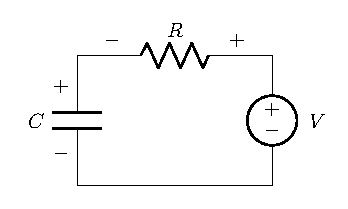
\includegraphics[width=\marginparwidth]{figures/tikz/3_rlc.pdf}}
        \caption{\scriptsize Circuito RC.}
        \label{fig:tikz-3_rlc-pdf}
    }
    Prendiamo il circuito RC come in figura \ref{fig:tikz-3_rlc-pdf}, l'equazione che regola la carica nel circuito è la seguente:
    \[
        \frac{\text{d} q}{\text{d} t} = \frac{V}{R}-\frac{q}{RC}
    .\] 
    In questo caso la variabile $x$ corrisponde con la carica.\\
    Il sistema non rispetta la condizione \ref{def:cond_lin}, infatti nello sviluppare il calcolo per due correnti, $q_1$ e $q_2$, rimane un termine $2V / R$. \\
    Nonostante questo il sistema è ancora lineare.
\end{exmp}
\noindent
\begin{exmp}[Pendolo]
    \marginpar{
        \captionsetup{type=figure}
            \incfig{1_9}
        \caption{\scriptsize }
        \label{fig:1_9}
    }
    Prendiamo il sistema del pendolo classico, le equazioni del moto della massa $m$ sono:
    \[
	\frac{\text{d} ^2\theta}{\text{d} t^2} = -\frac{g}{l}\sin\theta \implies
        \begin{cases}
	    \frac{\text{d} \theta}{\text{d} t} = y\\
	    \frac{\text{d} y}{\text{d} t} = - \frac{g}{l}\sin\theta
        \end{cases}
    .\] 
    Questo sistema è non lineare (c'è il seno).
\end{exmp}
\noindent
\begin{defn}[Criterio generale per la linearità]
    Un SD si dice lineare se la sua dipendenza dalle variabili di stato è lineare.
\end{defn}
\noindent
